\documentclass[12pt,a4paper]{article}
\usepackage[utf8]{inputenc}
\usepackage[T1]{fontenc}
\usepackage[polish]{babel}
\usepackage{amsmath}
\usepackage{graphicx}
\usepackage{float}
\usepackage{geometry}
\geometry{margin=2.5cm}

\title{Sprawozdanie: Algorytmy Metaheurystyczne -- Lista nr 2}
\author{Szymon Hładeżewski}
\date{\today}

\begin{document}

\maketitle

\section{Wprowadzenie}
Celem niniejszego sprawozdania jest analiza efektywności oraz prezentacja wyników działania dwóch popularnych metaheurystyk: algorytmu Symulowanego Wyżarzania (Simulated Annealing -- SA) oraz algorytmu Przeszukiwania z Tabu (Tabu Search -- TS). Both metody zostały zaimplementowane i przetestowane w kontekście rozwiązywania problemu komiwojażera (TSP).

Metoda symulowanego wyżarzania opiera się na analogii do procesów termodynamicznych zachodzących podczas chłodzenia ciał stałych. Kluczowym elementem jest parametr temperatury, który kontroluje poziom losowości w wyborze nowych stanów. Dzięki zastosowaniu kryterium akceptacji gorszych rozwiązań z prawdopodobieństwem określonym przez rozkład Boltzmanna $e^{(f(X)-f(X^{\prime}))/T}$, algorytm posiada zdolność do unikania przedwczesnej zbieżności i ucieczki z lokalnych optimów.

Z kolei algorytm Tabu Search stanowi rozwinięcie klasycznego przeszukiwania lokalnego. Wprowadza on pamięć krótkotrwałą w postaci listy tabu, na której zapisywane są niedawno wykonane ruchy. Zabronienie powrotu do tych samych stanów przez określoną liczbę iteracji skutecznie zapobiega cyklicznemu krążeniu wokół tych samych rozwiązań i wymusza eksplorację nowych obszarów przestrzeni.

\section{Metaheurystyka Symulowanego Wyżarzania}
\subsection{Analiza wpływu parametrów początkowych}
Pierwsza faza eksperymentów polegała na ocenie, jak parametry takie jak temperatura startowa oraz tempo jej spadku (współczynnik chłodzenia) wpływają na jakość końcowych rezultatów. Testy optymalizacyjne przeprowadzono na instancjach o różnej skali trudności.

\begin{figure}[H]
    \centering
    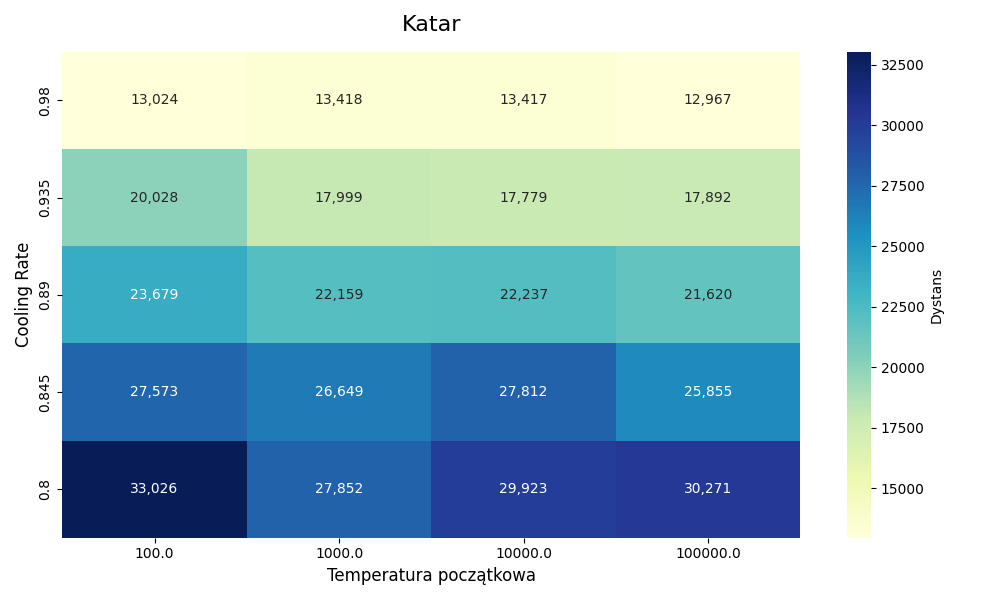
\includegraphics[width=0.8\textwidth]{../charts/Qatar1.png}
    \caption{Wpływ konfiguracji temperatury początkowej oraz współczynnika chłodzenia na wyniki końcowe dla instancji Katar (mapa cieplna).}
    \label{fig:sa_heatmap_qatar}
\end{figure}

\begin{figure}[H]
    \centering
    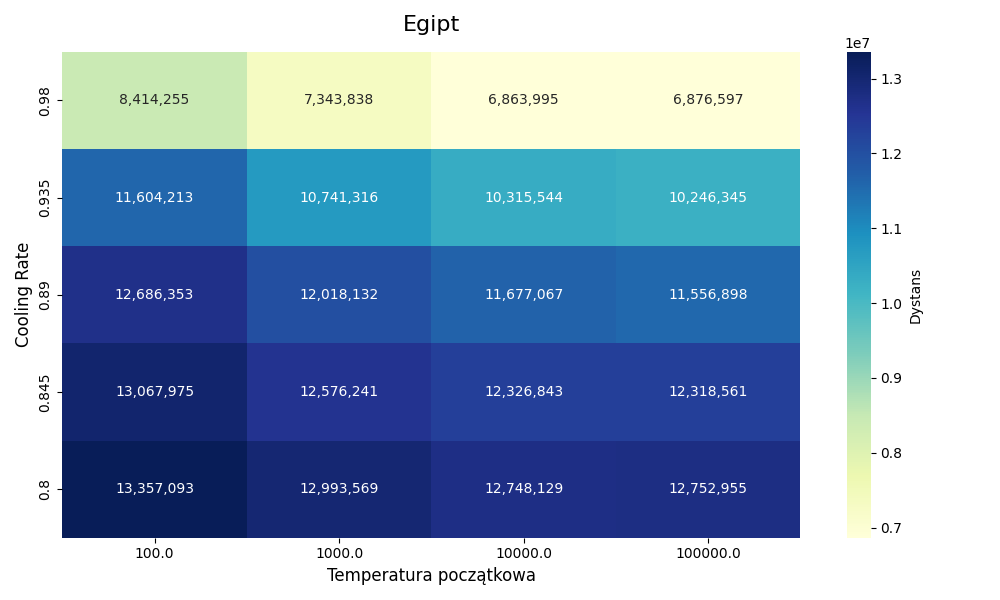
\includegraphics[width=0.8\textwidth]{../charts/Egipt1.png}
    \caption{Wizualizacja zależności uzyskanego dystansu od parametrów startowych algorytmu SA dla instancji Egypt.}
    \label{fig:sa_heatmap_egypt}
\end{figure}

W przypadku dużej instancji (Egipt), algorytm uruchomiono 100-krotnie dla wybranej konfiguracji, uzyskując następujące statystyki:
\begin{itemize}
    \item Najlepszy odnaleziony koszt trasy: 6 863 995
    \item Średni koszt rozwiązań z prób: 11 124 295.95
\end{itemize}

\begin{figure}[H]
    \centering
    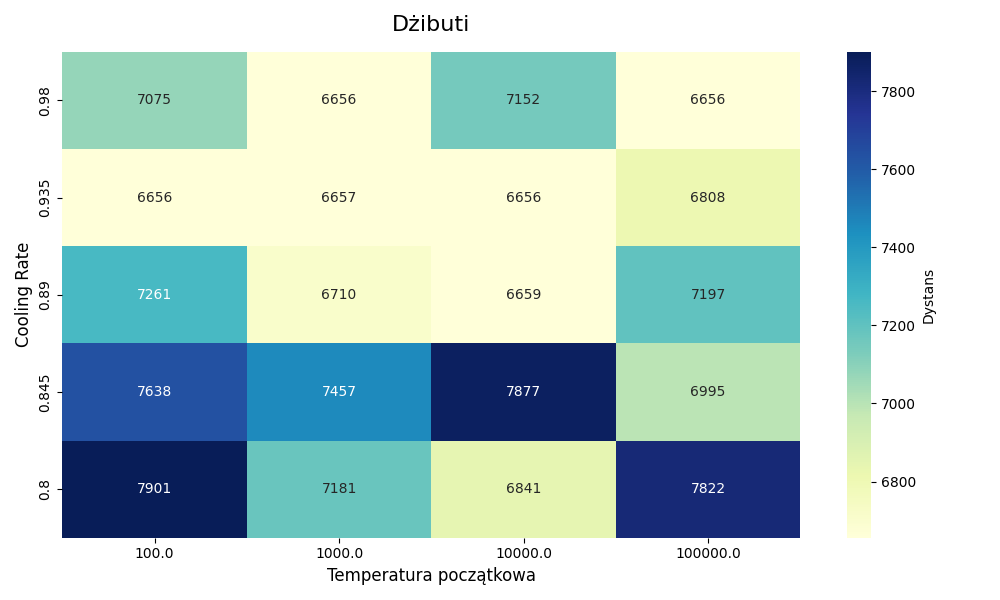
\includegraphics[width=0.8\textwidth]{../charts/Dzibuti1.png}
    \caption{Mapa zagęszczenia wyników algorytmu SA w przestrzeni parametrów dla instancji Djibouti.}
    \label{fig:sa_heatmap_djibouti}
\end{figure}

Analiza zgromadzonego materiału empirycznego przedstawionego na mapie cieplnej pozwala precyzyjnie wskazać konfiguracje, w których algorytm poprawnie zbiegał do optimum globalnego (osiągając wartość 6656). Odpowiednie zbalansowanie wysokiej temperatury z relatywnie szybkim tempem jej obniżania zaowocowało efektywnym przeszukiwaniem bez nadmiernego narzutu czasowego.

\section{Algorytm Tabu Search}
\subsection{Kalibracja parametrów algorytmu}
W przypadku algorytmu Tabu Search badaniom poddano dwa kluczowe parametry sterujące: długość kadencji na liście zabronień (\textit{tabu tenure}) oraz limit kroków bez odnotowania poprawy wyniku (\textit{max stagnation}), stanowiący warunek kryterium stopu.

\begin{figure}[H]
    \centering
    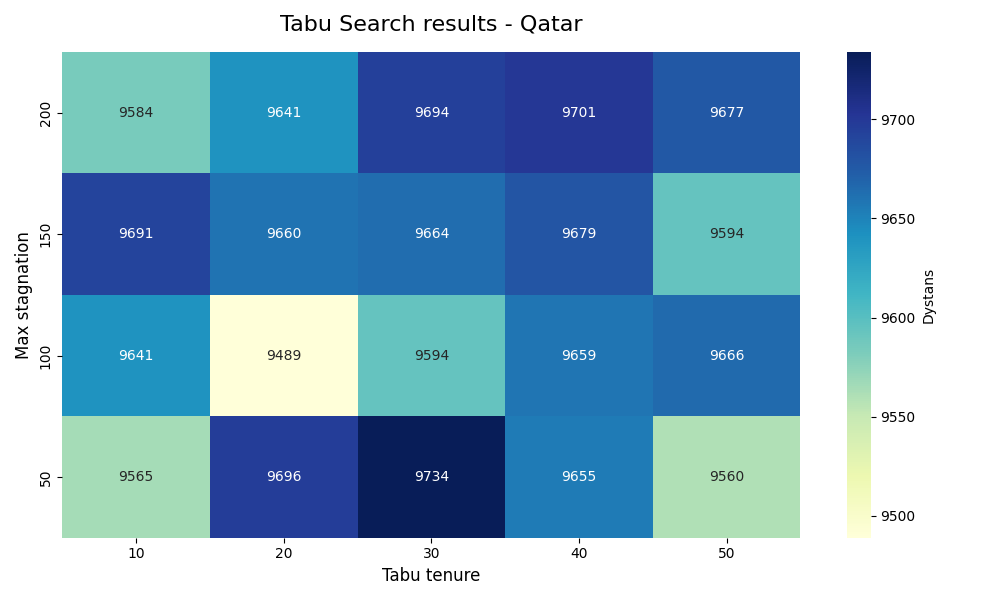
\includegraphics[width=0.8\textwidth]{../charts/Qatar2.png}
    \caption{Wpływ długości listy tabu oraz parametru stagnacji na długość wyznaczonej trasy w wariancie wykazującym zmienność.}
    \label{fig:ts_variable}
\end{figure}

Zgodnie z powyższym wykresem, najlepsze rezultaty (dystans na poziomie 9489) odnotowano przy zablokowaniu ruchów na 20 iteracji oraz dopuszczeniu 100 kroków stagnacji. Dalsze próby ujawniły jednak specyficzne zachowanie algorytmu, które zilustrowano na kolejnym wykresie -- w pewnych warunkach zmiana parametrów całkowicie traci wpływ na jakość rozwiązania.

\begin{figure}[H]
    \centering
    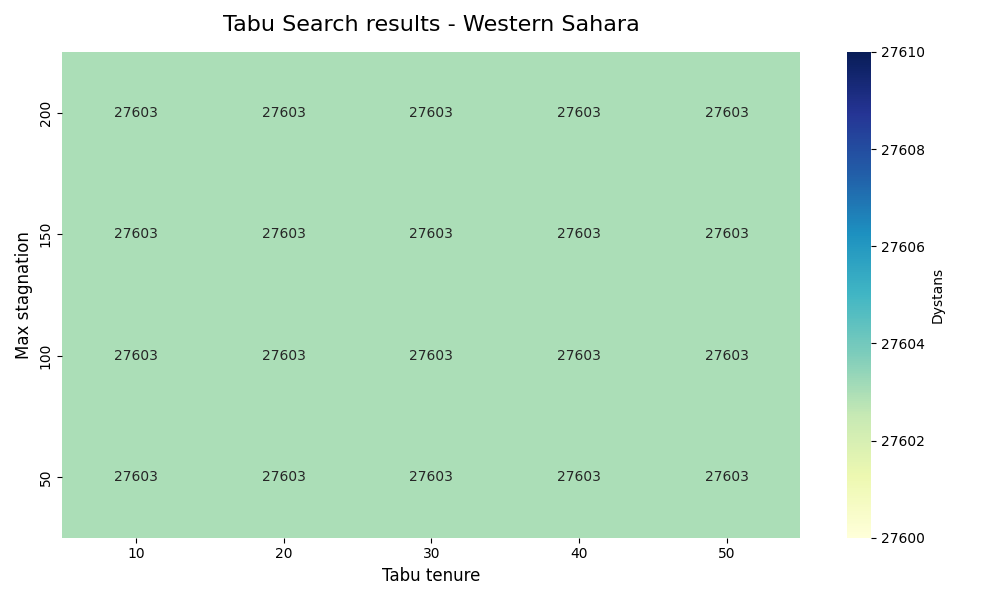
\includegraphics[width=0.8\textwidth]{../charts/WesternSahara.png}
    \caption{Zachowanie algorytmu Tabu Search przy braku wrażliwości na modyfikacje parametrów sterujących.}
    \label{fig:ts_uniform}
\end{figure}

Zjawisko generowania identycznych wyników końcowych przez algorytm Tabu Search dla mniejszych instancji testowych (np. Western Sahara) przy dowolnej konfiguracji parametrów można wytłumaczyć trzema zjawiskami:

\begin{enumerate}
    \item \textbf{Redukcja przestrzeni poszukiwań:} Ograniczona liczba wierzchołków determinuje niewielki i nieskomplikowany krajobraz rozwiązań. Algorytm bez trudu radzi sobie z taką strukturą danych, najprawdopodobniej każdorazowo odnajdując rzeczywiste minimum globalne problemu.
    
    \item \textbf{Podejście deterministyczne i kompletność otoczenia:} Strategia przeszukiwania zakłada pełną weryfikację sąsiedztwa o złożoności $\mathcal{O}(n^2)$ w każdym kroku. Dla małego grafu oznacza to błyskawiczną i powtarzalną zbieżność w stronę najgłębszego lokalnego zagłębienia, bez względu na wylosowany punkt startowy trasy.
    
    \item \textbf{Znikome znaczenie doboru parametrów:} Ponieważ optymalna ścieżka jest odnajdywana niemal natychmiast na początku obliczeń, podnoszenie progu \texttt{max\_stagnation} (np. z 50 do 200) wydłuża jedynie czas oczekiwania na stop, zmuszając algorytm do wykonywania bezproduktywnych iteracji wokół optymalnego stanu. Z kolei rozmiar pamięci \texttt{tabu\_tenure} jest na tyle duży w relacji do liczby miast, że całkowicie niweluje ryzyko zapętlenia.
\end{enumerate}

\textbf{Wnioski końcowe dla małych danych:} W środowisku o małej liczbie miast algorytm Tabu Search z pełnym przeglądem otoczenia cechuje się tak silną zbieżnością, że jego zachowanie staje się powtarzalne. Zmiany konfiguracji parametrów nie generują żadnych odchyleń w końcowej długości trasy.

\section{Komparatywna analiza metod i złożoności czasowej}
Końcowy etap badań stanowiło zestawienie sprawności oraz kosztów obliczeniowych zaimplementowanych metaheurystyk z metodami stworzonymi podczas realizacji wcześniejszego zadania.

Przeszukiwanie z listą tabu (Tabu Search) charakteryzuje się wyższą precyzją w odnajdywaniu dobrych stanów, jednak dzieje się to kosztem wyraźnie dłuższego czasu wykonywania programu w porównaniu do Symulowanego Wyżarzania. Większa dokładność TS przejawia się tym, że potrafi on wyznaczyć trasy o mniejszym całkowitym dystansie niż algorytm SA.

Jeżeli natomiast odniesiemy te wyniki do podejścia klasycznego, algorytm lokalnego przeszukiwania (Local Search) z poprzedniej listy okazuje się pod względem dokładności znacznie lepszy od algorytmu Tabu Search, aczkolwiek opłacone jest to olbrzymim narzutem i drastycznym spadkiem prędkości działania w stosunku do niego.

\end{document}